\section{Ambiente di lavoro}

Per il versionamento del codice e il coordinamento del gruppo è stato scelto di utilizzare \textbf{github}. Il progetto è stato infatti inserito e gestito all'interno di una repository \texttt{git}, in modo da controllare ogni singola modifica e rendere cooperativa la scrittura del codice.

Inoltre, per l'assegnazione dei task e il rilevamento dei bug è stato utilizzato il sistema di gestione delle \textit{issues}, che permette di gestire in modo molto efficace e ordinato il tutto, attraverso l'assegnazione ai vari membri e al filtraggio di quest'ultime tramite le etichette.

\begin{figure}[H]
		\centering 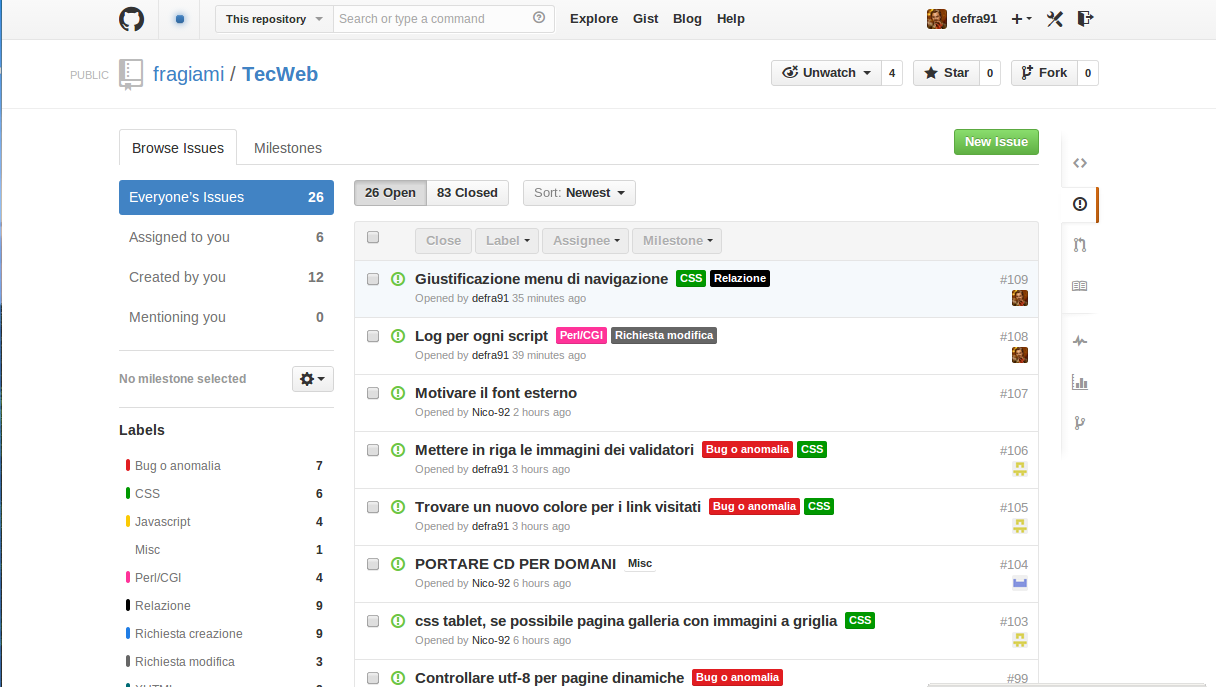
\includegraphics[width=0.8\textwidth]{images/github.png}
		\caption{Visualizzazione delle issues di github}
\end{figure}

Non è stato scelto un responsabile nel gruppo, quindi ciascuno si è preso la libertà di creare e assegnare issues a seconda delle necessità. Si è scelto un approccio molto \textit{agile} per lo sviluppo del progetto, in quanto, sebbene ritenuto molto rischioso per un gruppo poco esperto, ha lasciato un grado di libertà di gestione molto alto e ha quindi facilitato il lavoro di tutti a fronte dei diversi impegni sovrapposti. Nell'assegnazione delle issuess si è cercato di bilanciare il più possibile il lavoro fra i componenti del gruppo.

Ulteriori strumenti utilizzati sono riportati di seguito:

\begin{itemize}

	\item Come sistema operativo è stato utilizzato \textbf{Linux};
	\item Per la scrittura del codice si è scelto di utilizzare \textbf{Sublime Text 2};
	\item Come server-web di prova si è scelto di utilizzare \textbf{apache2};
	\item Per la gestione delle immagini si è utilizzato \textbf{Gimp};
	\item Per la stesura della relazione è stato utilizzato \textbf{\LaTeX\ };
	% STRUMENTI PER LA VALIDAZIONE???

\end{itemize}


